\section{Prior Work :  Dual View, Deep Gated Network, Role of Gates}\label{sec:prelim}
In this section, we make a briefly discuss the dual view, the deep gated network, and the main findings on the role of gates \citep{npk}.

\textbf{Dual View.} We consider a fully-DNN with `$d$' layers and  $w$  hidden units in each layer. The quantities `path feature' and `path value' in \Cref{sec:intro} will henceforth be called as \emph{neural path feature} (NPF) and \emph{neural path value} (NPV); these are defined in \Cref{def:npf-npv}. \Cref{prop:npf-npv} show that the output is the inner product of the NPF and NPV.
\begin{definition}\label{def:npf-npv}
A path starts from an input node, passes through a weight and a hidden unit in each layer and ends at the output node. We define the following quantities for a path $p$:
\emph{
\begin{tabular}{lcl}
 Activity&:& $A_{\Theta}(x,p)$ is the product of the `$d-1$' gates in the path. \\
Value&:& $v_{\Theta}(p)$ is the product of the `$d$' weights in the path.\\
Feature&:&   $\phi_{\Theta}(x,p)$ is the product of the signal at the input node of the path and $A_{\Theta}(x,p)$.\\
\end{tabular}
}

The \emph{neural path feature} (NPF) given by $\phi_{\Theta}(x)=\left(\phi_{\Theta}(x,p),p=1,\ldots, \Pfc\right),\in\R^{\Pfc}$ and the \emph{neural path value} (NPV) given by $v_{\Theta}=\left(v_{\Theta}(p),p=1,\ldots,\Pfc\right),\in\R^{\Pfc}$.
\end{definition}

\begin{proposition}\label{prop:npf-npv}
The output of the DNN is then the inner product of the NPF and NPV: 
\begin{align}\label{eq:inner}
\hat{y}_{\Theta}(x)=\ip{\phi_{\Theta}(x),v_{\Theta}}=\sum_{p\in[P]}  \phi_{\Theta}(x,p) v_{\Theta}(p)
\end{align}
\end{proposition}

\begin{figure}
\resizebox{1.0\columnwidth}{!}{
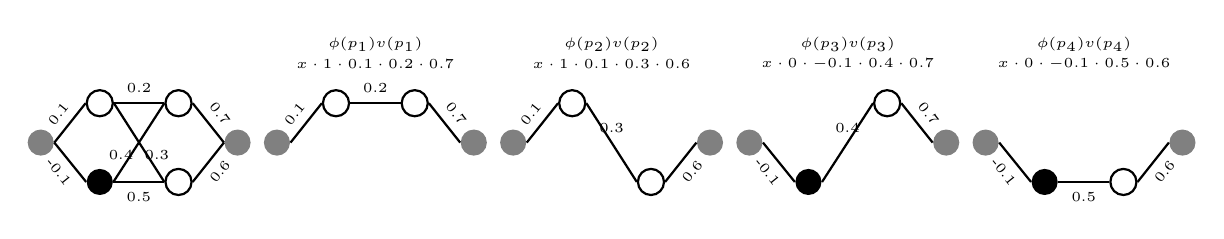
\begin{tikzpicture}
%Top Left
\node[draw,fill=white,circle,thick,
] (tl) at (-0.5,2){};

%Top Right
\node[draw,fill=white,circle,thick,
] (tr) at (0.5,2){};

%Bottom Left
\node[fill=black,circle,
] (bl) at (-0.5,1){};

%Bottom Right
\node[draw,fill=white,circle,thick,
] (br) at (0.5,1){};


%Input
\node[fill=gray,circle,
] (input) at (-1.25,1.5){};


%Output
\node[fill=gray,circle,
] (output) at (1.25,1.5){};

\draw[-, thick] (input.east) -- (tl.west) node [midway, above, sloped] (t1) {\tiny{0.1}};
\draw[-, thick] (input.east) -- (bl.west) node [midway, below, sloped] (t2) {\tiny{-0.1}};
\draw[-, thick] (tl.east) -- (tr.west) node [midway, above, sloped] (t1) {\tiny{0.2}};
\draw[-, thick] (bl.east) -- (br.west) node [midway, below, sloped] (t1) {\tiny{0.5}};
\draw[-, thick] (tl.east) -- (br.west) node [pos=0.85, above] (t1) {\tiny{0.3}};
\draw[-, thick] (bl.east) -- (tr.west) node [pos=0.15, above] (t1) {\tiny{0.4}};
\draw[-, thick] (tr.east) -- (output.west) node [midway, above, sloped] (t1) {\tiny{0.7}};
\draw[-, thick] (br.east) -- (output.west) node [midway, below, sloped] (t1) {\tiny{0.6}};




%%%%%%%%%%%%%%%%%Path 1%%%%%%%%%%%%%%
%Input
\node[fill=gray,circle,
] (p1input) at (1.75,1.5){};


%Output
\node[fill=gray,circle,
] (p1output) at (4.25,1.5){};



%Top Left
\node[draw,fill=white,circle,thick,
] (p1tl) at (2.5,2){};

%Top Right
\node[draw,fill=white,circle,thick,
] (p1tr) at (3.5,2){};




\draw[-, thick] (p1input.east) -- (p1tl.west) node [midway, above, sloped] (t1) {\tiny{0.1}};
\draw[-, thick] (p1tl.east) -- (p1tr.west) node [midway, above, sloped] (t1) {\tiny{0.2}};
\draw[-, thick] (p1tr.east) -- (p1output.west) node [midway, above, sloped] (t1) {\tiny{0.7}};



%%%%%%%%%%%%%%%%%Path 2%%%%%%%%%%%%%%

%Input
\node[fill=gray,circle,
] (p2input) at (4.75,1.5){};


%Output
\node[fill=gray,circle,
] (p2output) at (7.25,1.5){};

%Top Left
\node[draw,fill=white,circle,thick,
] (p2tl) at (5.5,2){};

%Bottom Right
\node[draw,fill=white,circle,thick,
] (p2br) at (6.5,1){};

\draw[-, thick] (p2input.east) -- (p2tl.west) node [midway, above, sloped] (t1) {\tiny{0.1}};
\draw[-, thick] (p2tl.east) -- (p2br.west) node [pos=0.5, above] (t1) {\tiny{0.3}};
\draw[-, thick] (p2br.east) -- (p2output.west) node [midway, below, sloped] (t1) {\tiny{0.6}};



%%%%%%%%%%%%%%%%%Path 3%%%%%%%%%%%%%%

%Input
\node[fill=gray,circle,
] (p3input) at (7.75,1.5){};


%Output
\node[fill=gray,circle,
] (p3output) at (10.25,1.5){};


%Top Right
\node[draw,fill=white,circle,thick,
] (p3tr) at (9.5,2){};

%Bottom Left
\node[fill=black,circle,
] (p3bl) at (8.5,1){};



\draw[-, thick] (p3input.east) -- (p3bl.west) node [midway, below, sloped] (t2) {\tiny{-0.1}};
\draw[-, thick] (p3bl.east) -- (p3tr.west) node [pos=0.5, above] (t1) {\tiny{0.4}};
\draw[-, thick] (p3tr.east) -- (p3output.west) node [midway, above, sloped] (t1) {\tiny{0.7}};


%%%%%%%%%%%%%%%%%Path 4%%%%%%%%%%%%%%

%Input
\node[fill=gray,circle,
] (p4input) at (10.75,1.5){};


%Output
\node[fill=gray,circle,
] (p4output) at (13.25,1.5){};

%Bottom Left
\node[fill=black,circle,
] (p4bl) at (11.5,1){};

%Bottom Right
\node[draw,fill=white,circle,thick,
] (p4br) at (12.5,1){};

\draw[-, thick] (p4input.east) -- (p4bl.west) node [midway, below, sloped] (t2) {\tiny{-0.1}};
\draw[-, thick] (p4bl.east) -- (p4br.west) node [midway, below, sloped] (t1) {\tiny{0.5}};
\draw[-, thick] (p4br.east) -- (p4output.west) node [midway, below, sloped] (t1) {\tiny{0.6}};
%%%%%%%%%%%%%%%%%%%%%%%%%%%%%%

\node[] () at (3,2.75){\tiny{$\phi(p_1)v(p_1)$}};
\node[] () at (3,2.5){\tiny{$x\cdot 1\cdot 0.1 \cdot 0.2 \cdot 0.7$}};

\node[] () at (6,2.75){\tiny{$\phi(p_2)v(p_2)$}};
\node[] () at (6,2.5){\tiny{$x\cdot 1\cdot 0.1 \cdot 0.3 \cdot 0.6$}};

\node[] () at (9,2.75){\tiny{$\phi(p_3)v(p_3)$}};
\node[] () at (9,2.5){\tiny{$x\cdot 0\cdot -0.1 \cdot 0.4 \cdot 0.7$}};

\node[] () at (12,2.75){\tiny{$\phi(p_4)v(p_4)$}};
\node[] () at (12,2.5){\tiny{$x\cdot 0\cdot -0.1 \cdot 0.5 \cdot 0.6$}};




\end{tikzpicture}


}
\end{figure}
\begin{comment}
\begin{figure}[t]
\centering
\resizebox{0.9\columnwidth}{!}{
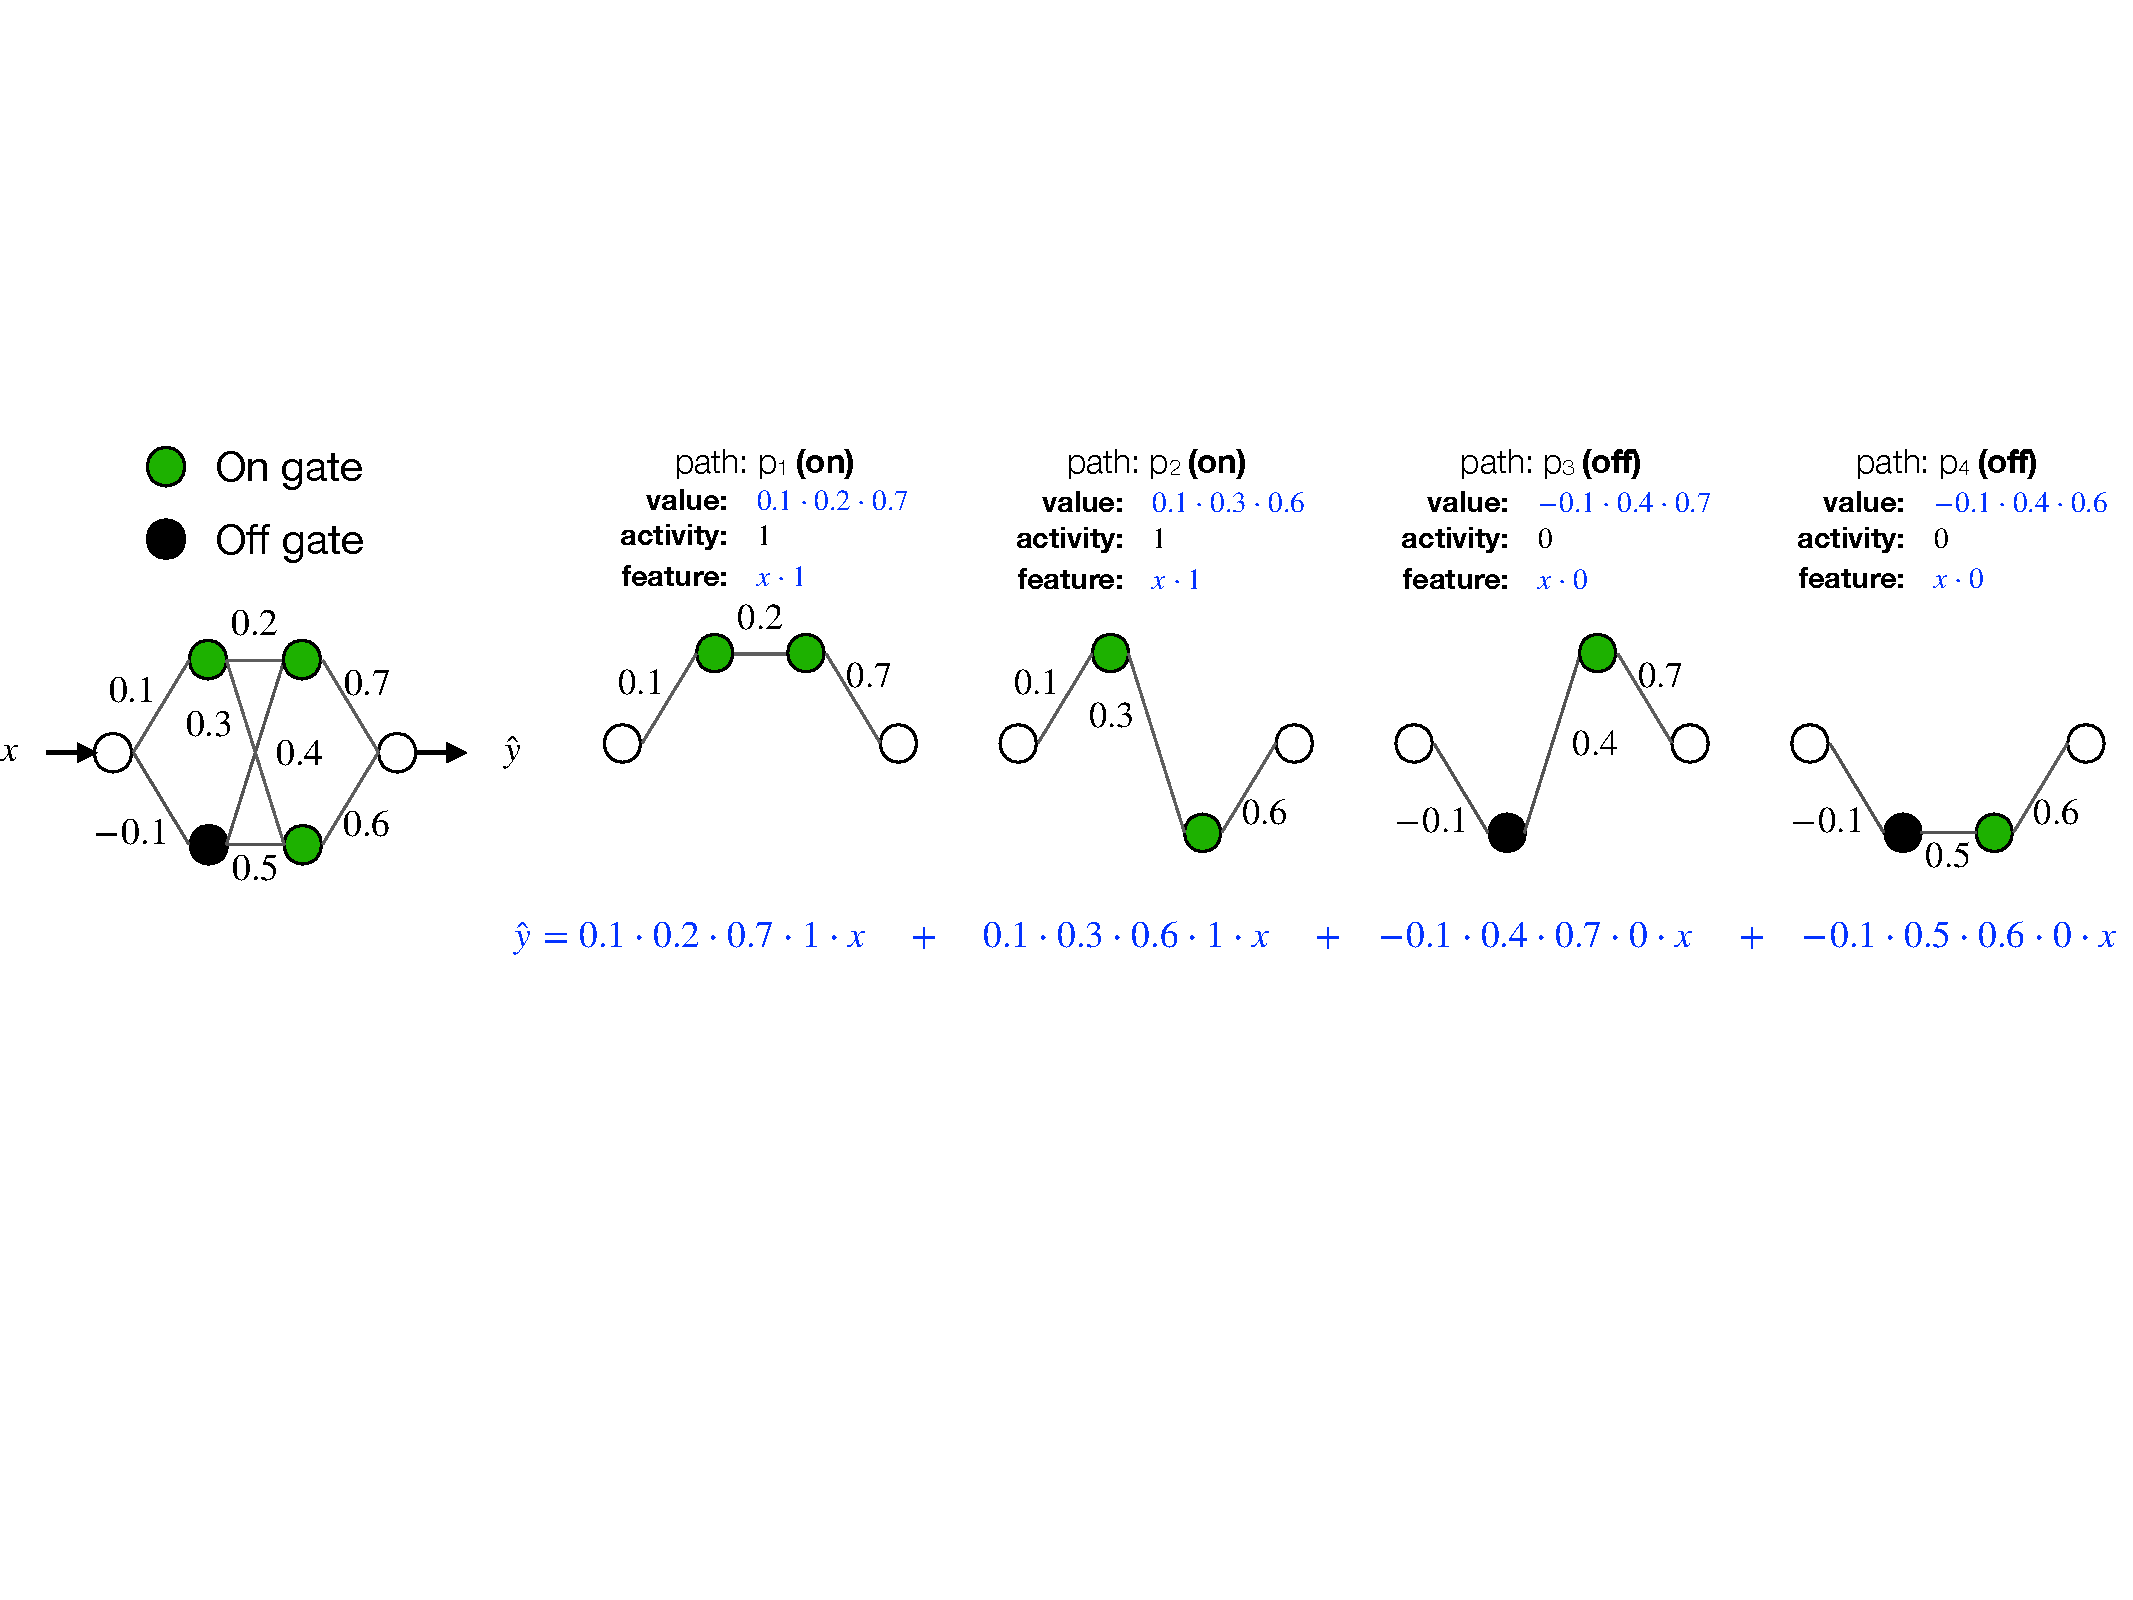
\includegraphics[scale=0.5]{figs/paths.pdf}
}
\caption{Illustration of \Cref{def:npf-npv} and \Cref{prop:npf-npv} in a  toy network with $2$ layers, $2$ gates per layer and $4$ paths. Paths $p_1$ and $p_2$ are `on' and paths $p_3$ and $p_4$ are `off'. The value, activity and feature of the individual paths are shown. $\hat{y}$ is the summation of the individual path contributions.}
\label{fig:paths}
\end{figure}

\begin{figure}
\centering
\begin{minipage}{0.8\columnwidth}
\begin{minipage}{0.49\columnwidth}
\resizebox{0.85\columnwidth}{!}{
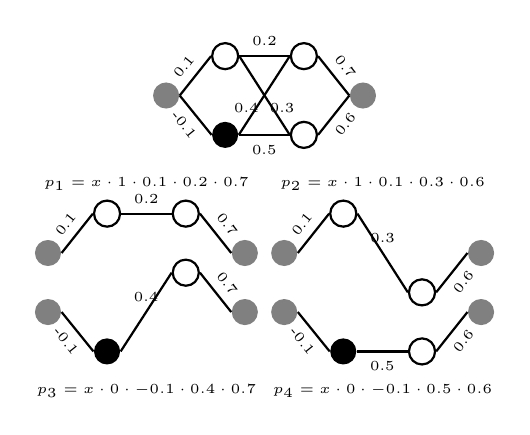
\begin{tikzpicture}
%Top Left
\node[draw,fill=white,circle,thick,
] (tl) at (-0.5,1.75){};

%Top Right
\node[draw,fill=white,circle,thick,
] (tr) at (0.5,1.75){};

%Bottom Left
\node[fill=black,circle,
] (bl) at (-0.5,0.75){};

%Bottom Right
\node[draw,fill=white,circle,thick,
] (br) at (0.5,0.75){};


%Input
\node[fill=gray,circle,
] (input) at (-1.25,1.25){};


%Output
\node[fill=gray,circle,
] (output) at (1.25,1.25){};

\draw[-, thick] (input.east) -- (tl.west) node [midway, above, sloped] (t1) {\tiny{0.1}};
\draw[-, thick] (input.east) -- (bl.west) node [midway, below, sloped] (t2) {\tiny{-0.1}};
\draw[-, thick] (tl.east) -- (tr.west) node [midway, above, sloped] (t1) {\tiny{0.2}};
\draw[-, thick] (bl.east) -- (br.west) node [midway, below, sloped] (t1) {\tiny{0.5}};
\draw[-, thick] (tl.east) -- (br.west) node [pos=0.85, above] (t1) {\tiny{0.3}};
\draw[-, thick] (bl.east) -- (tr.west) node [pos=0.15, above] (t1) {\tiny{0.4}};
\draw[-, thick] (tr.east) -- (output.west) node [midway, above, sloped] (t1) {\tiny{0.7}};
\draw[-, thick] (br.east) -- (output.west) node [midway, below, sloped] (t1) {\tiny{0.6}};




%%%%%%%%%%%%%%%%%Path 1%%%%%%%%%%%%%%
%Input
\node[fill=gray,circle,
] (p1input) at (-2.75,-0.750){};


%Output
\node[fill=gray,circle,
] (p1output) at (-0.25,-0.750){};



%Top Left
\node[draw,fill=white,circle,thick,
] (p1tl) at (-2.0,-0.25){};

%Top Right
\node[draw,fill=white,circle,thick,
] (p1tr) at (-1.0,-0.25){};




\draw[-, thick] (p1input.east) -- (p1tl.west) node [midway, above, sloped] (t1) {\tiny{0.1}};
\draw[-, thick] (p1tl.east) -- (p1tr.west) node [midway, above, sloped] (t1) {\tiny{0.2}};
\draw[-, thick] (p1tr.east) -- (p1output.west) node [midway, above, sloped] (t1) {\tiny{0.7}};



%%%%%%%%%%%%%%%%%Path 2%%%%%%%%%%%%%%

%Input
\node[fill=gray,circle,
] (p2input) at (0.25,-0.750){};


%Output
\node[fill=gray,circle,
] (p2output) at (2.75,-0.750){};

%Top Left
\node[draw,fill=white,circle,thick,
] (p2tl) at (1,-0.25){};

%Bottom Right
\node[draw,fill=white,circle,thick,
] (p2br) at (2,-1.25){};

\draw[-, thick] (p2input.east) -- (p2tl.west) node [midway, above, sloped] (t1) {\tiny{0.1}};
\draw[-, thick] (p2tl.east) -- (p2br.west) node [pos=0.5, above] (t1) {\tiny{0.3}};
\draw[-, thick] (p2br.east) -- (p2output.west) node [midway, below, sloped] (t1) {\tiny{0.6}};



%%%%%%%%%%%%%%%%%Path 3%%%%%%%%%%%%%%

%Input
\node[fill=gray,circle,
] (p3input) at (-2.75,-1.5){};


%Output
\node[fill=gray,circle,
] (p3output) at (-0.25,-1.5){};


%Top Right
\node[draw,fill=white,circle,thick,
] (p3tr) at (-1,-1){};

%Bottom Left
\node[fill=black,circle,
] (p3bl) at (-2,-2){};



\draw[-, thick] (p3input.east) -- (p3bl.west) node [midway, below, sloped] (t2) {\tiny{-0.1}};
\draw[-, thick] (p3bl.east) -- (p3tr.west) node [pos=0.5, above] (t1) {\tiny{0.4}};
\draw[-, thick] (p3tr.east) -- (p3output.west) node [midway, above, sloped] (t1) {\tiny{0.7}};


%%%%%%%%%%%%%%%%%Path 4%%%%%%%%%%%%%%

%Input
\node[fill=gray,circle,
] (p4input) at (0.25,-1.50){};


%Output
\node[fill=gray,circle,
] (p4output) at (2.75,-1.50){};

%Bottom Left
\node[fill=black,circle,
] (p4bl) at (1,-2){};

%Bottom Right
\node[draw,fill=white,circle,thick,
] (p4br) at (2,-2){};

\draw[-, thick] (p4input.east) -- (p4bl.west) node [midway, below, sloped] (t2) {\tiny{-0.1}};
\draw[-, thick] (p4bl.east) -- (p4br.west) node [midway, below, sloped] (t1) {\tiny{0.5}};
\draw[-, thick] (p4br.east) -- (p4output.west) node [midway, below, sloped] (t1) {\tiny{0.6}};


%%%%%%%%%%%%%%%%%%%%%%%%%%%%%%%%%%%%%%%%%%%%

\node[] () at (-1.5,0.125){\tiny{$p_1=x\cdot 1\cdot 0.1 \cdot 0.2 \cdot 0.7$}};

\node[] () at (1.5,0.125){\tiny{$p_2=x\cdot 1\cdot 0.1 \cdot 0.3 \cdot 0.6$}};

\node[] () at (-1.5,-2.5){\tiny{$p_3=x\cdot 0\cdot -0.1 \cdot 0.4 \cdot 0.7$}};

\node[] () at (1.5,-2.5){\tiny{$p_4=x\cdot 0\cdot -0.1 \cdot 0.5 \cdot 0.6$}};




\end{tikzpicture}


}
\end{minipage}
\begin{minipage}{0.49\columnwidth}
\resizebox{0.99\columnwidth}{!}{
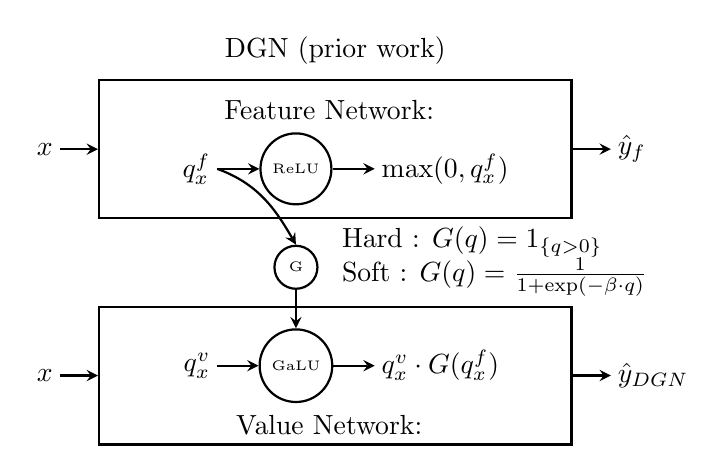
\begin{tikzpicture}

\node []  (fntext)at (3.5,1.5) {DGN (prior work)};
%Feature Network
\node [draw,
	minimum width=6cm,
	minimum height=1.75cm,
	thick
]  (fnbox)at (3.5,0.25) {};
\node []  (fntext)at (3.5,0.75) {Feature Network: $\Tf$};


%Feature Network Input
\node (fin) [left of=fnbox,node distance=3.5cm, coordinate] {};
\node[left=-1pt] at (fin.west){$x$};
\draw[-stealth, thick] (fin.center) -- (fnbox.west);

%Feature Network Output
\node (fout) [right of=fnbox,node distance=3.5cm, coordinate] {};
\node[right=-1pt] at (fout.west){$\hat{y}_{\text{f}}$};
\draw[-stealth, thick]  (fnbox.east)--(fout.center);


%ReLU Circle
\node[draw,
	circle,
	minimum size=0.75cm,thick,
] (relu) at (3,0){\tiny{ReLU}};
%ReLU Input
\node (b) [left of=relu,node distance=1cm, coordinate] {};

\node[left=-1pt] at (b.center){$q^\text{f}_x$};
\draw[-stealth, thick] (b.east) -- (relu.west);


%ReLU Output
\node (c) [right of=relu,node distance=1cm, coordinate] {};
\node[right=-1pt] at (c.center){$\max(0,q^\text{f}_x)$};
\draw[-stealth, thick] (relu.east) -- (c.west);
	

%Gating Circle
\node[draw,
	circle,
	minimum size=0.0625cm,thick,
] (gating) at (3,-1.25){\tiny{G}};
%\node[right=6pt] at (gating.north){Hard : $G(q)=\mathbbm{1}_{\{q>0\}} $};
%\node[below right=6pt] at (gating.north){Soft : $G(q)=\frac{1}{1+\exp(-\beta\cdot q)}$};

\node[right=6pt] at (3.25,-0.925){Hard : $G(q)=\mathbbm{1}_{\{q>0\}} $};
\node[right=6pt] at (3.25,-1.375){Soft : $G(q)=\frac{1}{1+\exp(-\beta\cdot q)}$};


%Value Network

\node [draw,
	minimum width=6cm,
	minimum height=1.75cm,
	thick
]  (vnbox)at (3.5,-2.625) {};

\node []  (vntext)at (3.5,-3.25) {Value Network: $\Tv$};

%Value Network Input
\node (vin) [left of=vnbox,node distance=3.5cm, coordinate] {};
\node[left=-1pt] at (vin.west){$x$};
\draw[-stealth, thick] (vin.center) -- (vnbox.west);

%Feature Network Input
\node (vout) [right of=vnbox,node distance=3.5cm, coordinate] {};
\node[right=-1pt] at (vout.west){$\hat{y}_{\text{DGN}}$};
\draw[-stealth, thick]  (vnbox.east)--(vout.center);



%GaLU Circle
\node[draw,
	circle,
	minimum size=0.75cm,thick,
] (galu) at (3,-2.5){\tiny{GaLU}};

\draw [-stealth,thick]   (b) to[out=-20,in=120] (gating.north);
\draw [-stealth,thick]   (gating.south) -- (galu.north);


%GaLU Input
\node (d) [left of=galu,node distance=1cm, coordinate] {};
\node[left=-1pt] at (d.center){$q^\text{v}_x$};
\draw[-stealth, thick] (d.east) -- (galu.west);
%GaLU Output
\node (e) [right of=galu,node distance=1cm, coordinate] {};
\node[right=-1pt] at (e.center){$q^\text{v}_x\cdot G(q^\text{f}_x)$};
\draw[-stealth, thick] (galu.east) -- (e.west);
	
\end{tikzpicture}


}
\end{minipage}
\end{minipage}
\caption{DGN}
\label{fig:dgn}
\end{figure}
\end{comment}
%As mentioned in \Cref{sec:intro}, a deep gated network(DGN) setup is an alternative way to compute path-by-path, that is, the to compute the inner product of the neural path feature and neural path value. In this section, we first describe DGN in prior work \citep{npk}:  consitituent parts, information flow, purpose and training. We then discuss the two fundamental conceptual issues that make this DGN `black box'. We then present our modified \texttt{DGN-NO-ACT} with an intutitve explanation of how the conceptual issues are overcome and  why it is an entirely interpretatble white box model. These intuitive explanations will be justified in theory and experiments in \Cref{sec:main}.

\textbf{Deep Gated Network (DGN)} is an alternative way to compute the inner product of the neural path feature and neural path value. Consider a DNN with ReLUs with weights $\Theta\in\R^{\dnet}$. The DGN \emph{corresponding} to this DNN (see the left diagram in \Cref{fig:dgn}) has two networks of \emph{identical archicture} (to the DNN) namely the feature network and value network with distinct weights $\Tf\in\R^{\dnet}$ and $\Tv\in\R^{\dnet}$ respectively. The main difference between the feature and value networks is in the activations. The feature network has ReLUs which turn `on/off' based on their pre-activation signal, and the value  network has gated linear units (GaLUs) \citep{sss,npk}. Each GaLU multiplies its pre-activation input by an external gating signal. Since the feature and value networks have identical architecture, there is an one-to-one correspondance between the ReLUs and GaLUs in the respective networks.
In the DGN, the external gating signal to the GaLU is derived from the pre-activation input of the corresponding ReLU. The feature network deals with the primal layer-by-layer computations, the pre-activations from the feature network generate the gates, which are then used to switch `on/off' the corresponding GaLUs in the value network: this realises $\phi_{\Tf}(x)$. The value network realises $v_{\Tv}$ and computes the output $\hat{y}_{\text{DGN}}(x)=\ip{\phi_{\Tf}(x),v_{\Tv}}$.

\subsection{Information in the Gates/Neural Path Features: Motivation and Key Results}

During training, a DNN learns the relation $\hat{y}(x)=\ip{\phi_\Theta(x),v_\Theta}$, i.e., it learns both the neural path features and value. The DGN separately store $\phi(x)$ and $v$ in the feature and value network respectively and helps in understanding their roles separately. Using the DGN, the following  were answered:



{\centering \emph{{Do $\phi(x)$s behave like features? Or Given the features $\phi(x)$s can we learn $v$?}}\par}

This is answered by operating the DGN in the \textbf{fixed learnt (FL)} mode. Here, the feature network (which is a DNN with ReLU) is \emph{pre-trained} with $\hat{y}_f$ as the output. Then the feature network is frozen and the value network is trained, i.e., in $\hat{y}_{\text{DGN}}(x)=\ip{\phi_{\Tf}(x),v_{\Tv}}$, $\phi_{\Tf}(x)$ is fixed and only $v_{\Tv}$ is learnt. Here, `hard'-gating is used: for pre-activation $q\in\R$, the gating value is $G(q) = \mathbbm{1}_{\{q>0\}}$. It was shown that \emph{most useful information is in the gates/neural path features}, i.e., using a pre-trained DNN as feature network, we can train the value network separately from scratch and match the performance of the pre-trained DNN. In other words, using pre-trained $\phi_{\Tg}(x)$ we can train the $v_{\Tv}$, in a manner analogous to linear models wherein given the features we can train the weights. 


{\centering \emph{{Are $\phi(x)$s learnt during training? If so, how important is such learning?}}\par}

This is answered by operating the DGN in the \textbf{fixed random (FR)} mode, which is similar to the FL mode, expect that, in the FR mode the feature network is randomly initialised and kept frozen, and only the value network is trained. Here too, hard gating is used. It was shown that  random gates/neural path features perform significantly poorly than the learnt gates/neural path features. Using the previous result that the learnt gates/neural path features perform as well as the trained DNN, it was concluded that the $\phi(x)$s are learnt during training and such learning is key for generalisation.

{\centering \emph{{Can $\phi(x)$s and $v$ be learnt  separately? or How good is a DGN compared to DNN?}}\par}

This is answered by operating the DGN in the \textbf{decoupled learning (DL)} mode, wherein, both the feature and value networks are trained starting from random initialisation. Here, `soft'-gating is used, where, $G(q)=\frac{1}{1+\exp({-\beta\cdot q})}$ ($\beta=10$ is a typical choice): this enables gradient to flow via the feature network. It was shown that DGN performs only marginally poorly compared to a DNN.

{\centering \emph{{What is the analytical characterisation of the information in the gates/neural path features?}}\par}

Prior work by \cite{ntk,arora2019exact,cao2019generalization} showed that training an infinite width DNN is equivalent to a kernel method with the so called \emph{neural tangent kernel} (NTK). \citep{npk} showed that in an infinite width fully connected DGN with its gates fixed, the NTK is equal (up to a scalar) to the so called \emph{neural path kernel} (NPK) (equal to the Gram matrix of the neural path features). 



%\textbf{DGN Training.} The primary use of the DGN was to measure the information in the gates of a DNN with ReLU. For this, the feature network (which is a DNN with ReLU) is \emph{pre-trained} with $\hat{y}_f$ as the output. Then the feature network is frozen and the value network is trained, i.e., in $\hat{y}_{\text{DGN}}(x)=\ip{\phi_{\Tf}(x),v_{\Tv}}$, $\phi_{\Tf}(x)$ is fixed and only $v_{\Tv}$ is learnt. Here, `hard'-gating is used: for pre-activation $q\in\R$, the gating value is $G(q) = \mathbbm{1}_{\{q>0\}}$. The secondary use of DGN is as an alternative/competetive model (for DNN) that learns  $\hat{y}_{\text{DGN}}(x)=\ip{\phi_{\Tf}(x),v_{\Tv}}$, by separately learning $\Tf$ and $\Tv$ starting from randomised initialisation.Here, `soft'-gating is used, where, $G(q)=\frac{1}{1+\exp({-\beta\cdot q})}$ ($\beta=10$ is a typical choice): this enables gradient to flow via the feature network. 


\begin{comment}
\begin{definition}[Overlap of active sub-networks]\label{def:overlap} 
The total number of `active' paths for both $x$ and $x'$ that pass through input node $i$ is defined to be:\\
{\centering{\centering{$\textbf{overlap}_{\Theta}(i,x,x') = \Lambda_{\Theta}(i,x,x') \eqdef \left|\{p \colon  A_{\Theta}(x,p)= A_{\Theta}(x',p)=1\}\right|/\din$}}}
\end{definition}
%\subsection{NPK of FC-DNN: Product Kernel }
%\input{cnpkexample}
%\subsection{Neural Path Kernel : Similarity based on active sub-networks}
\begin{lemma}[Neural Path Kernel (NPK)]\label{lm:npk}
Let $D\in\R^{\din}$ be a vector of non-negative entries  and for $u,u'\in\R^{\din}$ , let $\ip{u,u'}_{D}=\sum_{i=1}^{\din}D(i)u(i)u'(i)$. Let $H_{\Theta}(x,x')\eqdef\langle\phi_{\Theta}(x),\phi_{\Theta}(x') \rangle$ be the neural path kernel (NPK). Then  
\begin{align*} 
\text{NPK}_{\Theta}(x,x')= H_{\Theta}(x,x')=\ip{x,x'}_{\Lambda_{\Theta}(\cdot,x,x')} 
\end{align*}
\end{lemma}
\textbf{Remark.} In the case of fully connected networks, $\textbf{overlap}_{\Theta}(i,x,x')$ is equal for all $i\in[\din]$, and hence $\text{NPK}_{\Theta}(x,x')=\ip{x,x'}\cdot\textbf{overlap}_{\Theta}(x,x')$.
\end{comment}
